\section{General Information}
All submitted paper to some SBC conference, including any supporting
documents, should be written in English or in Portuguese. The format
paper should be A4 with single column, 3.5~cm for upper margin, 2.5~cm
for bottom margin and 3.0~cm for lateral margins, without headers or
footers. The main font must be Times, 12~point nominal size, with
6~points of space before each paragraph. Page numbers must be
suppressed in the final version.

Teste de bibliografia \cite{Dean2008}.

Full papers must respect the page limits defined by the conference.
Conferences that publish just abstracts ask for \textbf{one}-page
texts.

\section{First Page}
The first page must display the paper title, the name and address of
the authors, the abstract in English and ``resumo'' in Portuguese (for
papers written in Portuguese). The title must be justified at the
left, in 20~point boldface font. Author names must be justified in the
same way, as shown in this example.

\section{CD-ROMs and Printed Proceedings}
In some conferences, the papers are published on CD-ROM while only the
abstract is published in the Proceedings. In this case, authors are
invited to prepare two final versions of the paper. One, complete, to
be published on the CD and the other, containing only the first page,
with abstract and ``resumo'' (for papers in Portuguese).

\section{Sections and Paragraphs}
Section titles must be in boldface, 13pt, flush left. There should be
an extra 12~pt of space before each title. The first paragraph of each
section should not be indented; the first lines of subsequent
paragraphs should be indented by 1.27~cm.

\subsection{Subsections}
The subsection titles must be in boldface, 12pt, flush left.

\section{Figures and Captions}
\label{sec:captionmargins}
Figures and tables captions should be centered if less than one line
(Figure~\ref{figone}), otherwise justified and indented by 0.8cm on
both margins, as shown in Figure~\ref{figtwo}. The font must be
Helvetica, 10~point, boldface, with 6~points of space before and after
each caption.

\begin{figure}[h!]
	\centerline{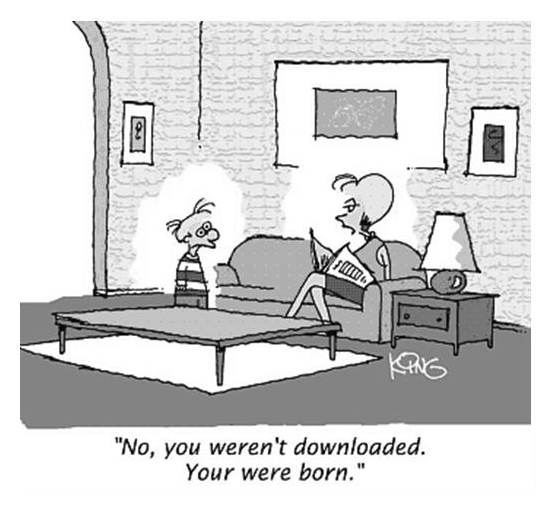
\includegraphics{fig1}}
	\caption{A typical figure}
	\label{figone}
\end{figure}

In tables, do not use colored or shaded backgrounds, and avoid thick,
doubled, or unnecessary framing lines. When reporting empirical data,
do not use more decimal digits than warranted by their precision and
reproducibility. Table caption must be placed before the table (see
Table~\ref{tabone}) and the font used must also be Helvetica,
10~point, boldface, with 6~points of space before and after each
caption.

Figure and table references must be composed by the chapter number and
a sequence number beginning in one (see the examples of
Figure~\ref{figone}, Figure~\ref{figtwo} and Table~\ref{tabone}).

\begin{figure}[h!]
	\centerline{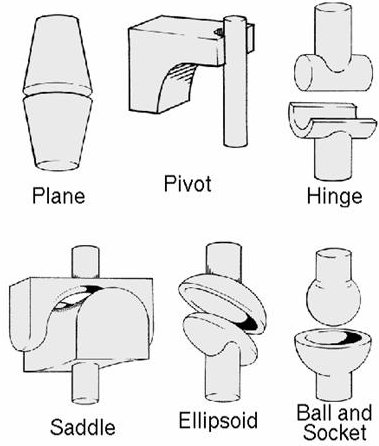
\includegraphics{fig2}}
	\caption{This figure is an example of a figure caption taking
		more than one line and justified considering margins
		mentioned in Section~\ref{sec:captionmargins}}
	\label{figtwo}
\end{figure}

\section{Images}
All images and illustrations should be in black-and-white, or gray
tones. The image resolution on paper should be about 600~dpi for
black-and-white images, and 150-200~dpi for grayscale images.  Do not
include images with excessive resolution, as they may take hours to
print, without any visible difference in the result.

\begin{table}[h!]
	\caption{Variables to be considered on the evaluation of
		interaction techniques.}
	\label{tabone}
	\begin{footnotesize}
	\begin{tabular}{|p{40mm}|p{55mm}|p{42mm}|}
	\hline
	\hspace*{\fill}\textbf{Tarefa}\hspace*{\fill} &
	\hspace*{\fill}\textbf{Variável}\hspace*{\fill} & 
	\hspace*{\fill}\textbf{Métrica utilizada}\hspace*{\fill}\\
	\hline
	Sele{'c}{~a}o &
	Distancia do alvo &
	Virtual cubits \\ \cline{2-3}
	& Dire{'c}{~a}o horizontal e vertical do alvo &
	Graus do arco \\ \cline{2-3}
	& Distancia do objeto oculto &
	Virtual cubits \\ \cline{2-3}
	& Direcao da oclusao &
	Esquerda/direita/cima/baixo \\
	\hline
	Posicionamento &
	Distancia inicial &
	Virtual cubits \\ \cline{2-3}
	& Direcoes iniciais horizontal e vertical &
	Graus do arco \\ \cline{2-3}
	& Distancia final &
	Virtual cubits \\ \cline{2-3}
	& Direcoes finais horizontal e vertical &
	Graus do arco \\ \cline{2-3}
	& Precisao vertical &
	Porcentagem de sobreposicao \\ \cline{2-3}
	& Precisao horizontal &
	Porcentagem de sobreposicao \\
	\hline
	Orientacao &
	Distancia &
	Virtual cubits \\ \cline{2-3}
	& Direcoes horizontal e vertical &
	Graus do arco \\ \cline{2-3}
	& Orientacao inicial (3 angulos) &
	Graus do arco \\ \cline{2-3}
	& Orientacao final (3 angulos) &
	Graus do arco \\ \cline{2-3}
	& Exatidao/precisao &
	Graus do arco \\
	\hline
	\end{tabular}
	\end{footnotesize}
\end{table}

